\subsection{Outcome modelling}

\subsubsection{Modified Rankin scale}

We used modified Rankin Scale (mRS) at 6 months as a measure of outcome. mRS is the most commonly used instrument to describe post-stroke functional outcome \cite{quinn_functional_2009}, describing independence of living from a scale of 0 (no disability) through to 5 (severe disability requiring constant nursing attention), with death assigned an mRS of 6. A commonly used surrogate for independent living is  mRS 0-2. Health utility values for each mRS level were taken from Wang \textit{et al.} \cite{wang_utility-weighted_2020}. These were 0.0, -0.19, 0.20, 0.55, 0.74, 0.88 and 0.97 for mRS 0-6. The mean mRS score, mean utility and proportion of patients with mRS 0-2 in a given mRS distribution can be compared between scenarios. Table \ref{tab:mrs} shows a description of each mRS category.

\begin{minipage}{1.0\textwidth}  % Define the width of the minipage
\begin{longtable}{p{1.2cm} p{13cm}}
\caption{Description of modified Rankin Scale (mRS)categories}\label{tab:mrs}\\
\toprule
mRS & Description \\
\midrule
0 & No symptoms. \\
1 & No significant disability. Able to carry out all usual activities,
despite some symptoms. \\
2 & Slight disability. Able to look after own affairs without
assistance, but unable to carry out all previous activities. \\
3 & Moderate disability. Requires some help, but able to walk
unassisted. \\
4 & Moderately severe disability. Unable to attend to own bodily needs
without assistance, and unable to walk unassisted. \\
5 & Severe disability. Requires constant nursing care and attention,
bedridden, incontinent. \\
6 & Dead. \\
\bottomrule
\end{longtable}
\end{minipage} 
6.

\subsubsection{Treatment of ischaemic stroke}

Reperfusion treatment aims to  the restoration of blood flow following an ischaemic stroke. There are two potential reperfusion treatments:

\begin{itemize}
    \item \textit{Thrombolysis} (also known as as intravenous thrombolysis, IVT) is a medical therapy where clot-busting drugs are used to reduce or remove the blood clot. It is potentially of use in both nLVO and LVO.
    
    \item \textit{Thrombectomy} (also known as mechanical thrombectomy, MT) is the physical removal of a clot, by a mesh device under image guidance. Thrombectomy is suitable only for clots in a large vessel (these generally cause the worst strokes). It is potentially of use in LVO.
\end{itemize}


\subsubsection{Outcome modelling overview}

Detailed methods and code used for modelling these outcomes are available \cite{github2}, with methods described as an online book \cite{github3}. The outcome model is available as a PyPI package for Python \cite{pypi}.

We used modified Rankin Scale (mRS) at 3-6 months as a measure of outcome. mRS is the most commonly used instrument to describe post-stroke functional outcome \cite{quinn_functional_2009}, describing independence of living from a scale of 0 (no disability) through to 5 (severe disability requiring constant nursing attention), with death assigned an mRS of 6. A commonly used surrogate for independent living is  mRS 0-2. Health utility values for each mRS level were taken from Wang \textit{et al.} \cite{wang_utility-weighted_2020}. The mean mRS score, mean utility and proportion of patients with mRS 0-2 in a given mRS distribution can be compared between scenarios.

We calculated the patients mRS outcome distribution based on time to treatment for three patient-treatment cohorts: nLVO treated with IVT; LVO treated with IVT alone; and LVO treated with IVT and MT. For each patient-treatment cohort we calculated an mRS distribution for treatment at any given time by interpolating between the mRS distribution for treatment given at \emph{t=0} (time of stroke onset) and the mRS distribution for treatment given at \emph{t=No Effect} (time of no effect of treatment), assuming that log odds fall linearly over time \cite{emberson_effect_2014, fransen_time_2016}.

The time to no effect was 6.3 hours for IVT \cite{emberson_effect_2014} and 8.0 hours for MT \cite{ fransen_time_2016}. Our model did not include selection of patients who may still benefit from treatment beyond these durations through the use of perfusion scanning. This number is small for IVT, but is more substantial for MT – approximately 2,500 per annum in England. 

The model synthesises data from multiple sources (figure \ref{fig:data_cauldron}) including reperfusion treatment clinical trials and nationals stroke audit data for England and Wales. Predictions from the combined model are then compared against original clinical trials and other models. Details of how these data are synthesised are given in the sections below.

\begin{figure}[h!]
    \centering
    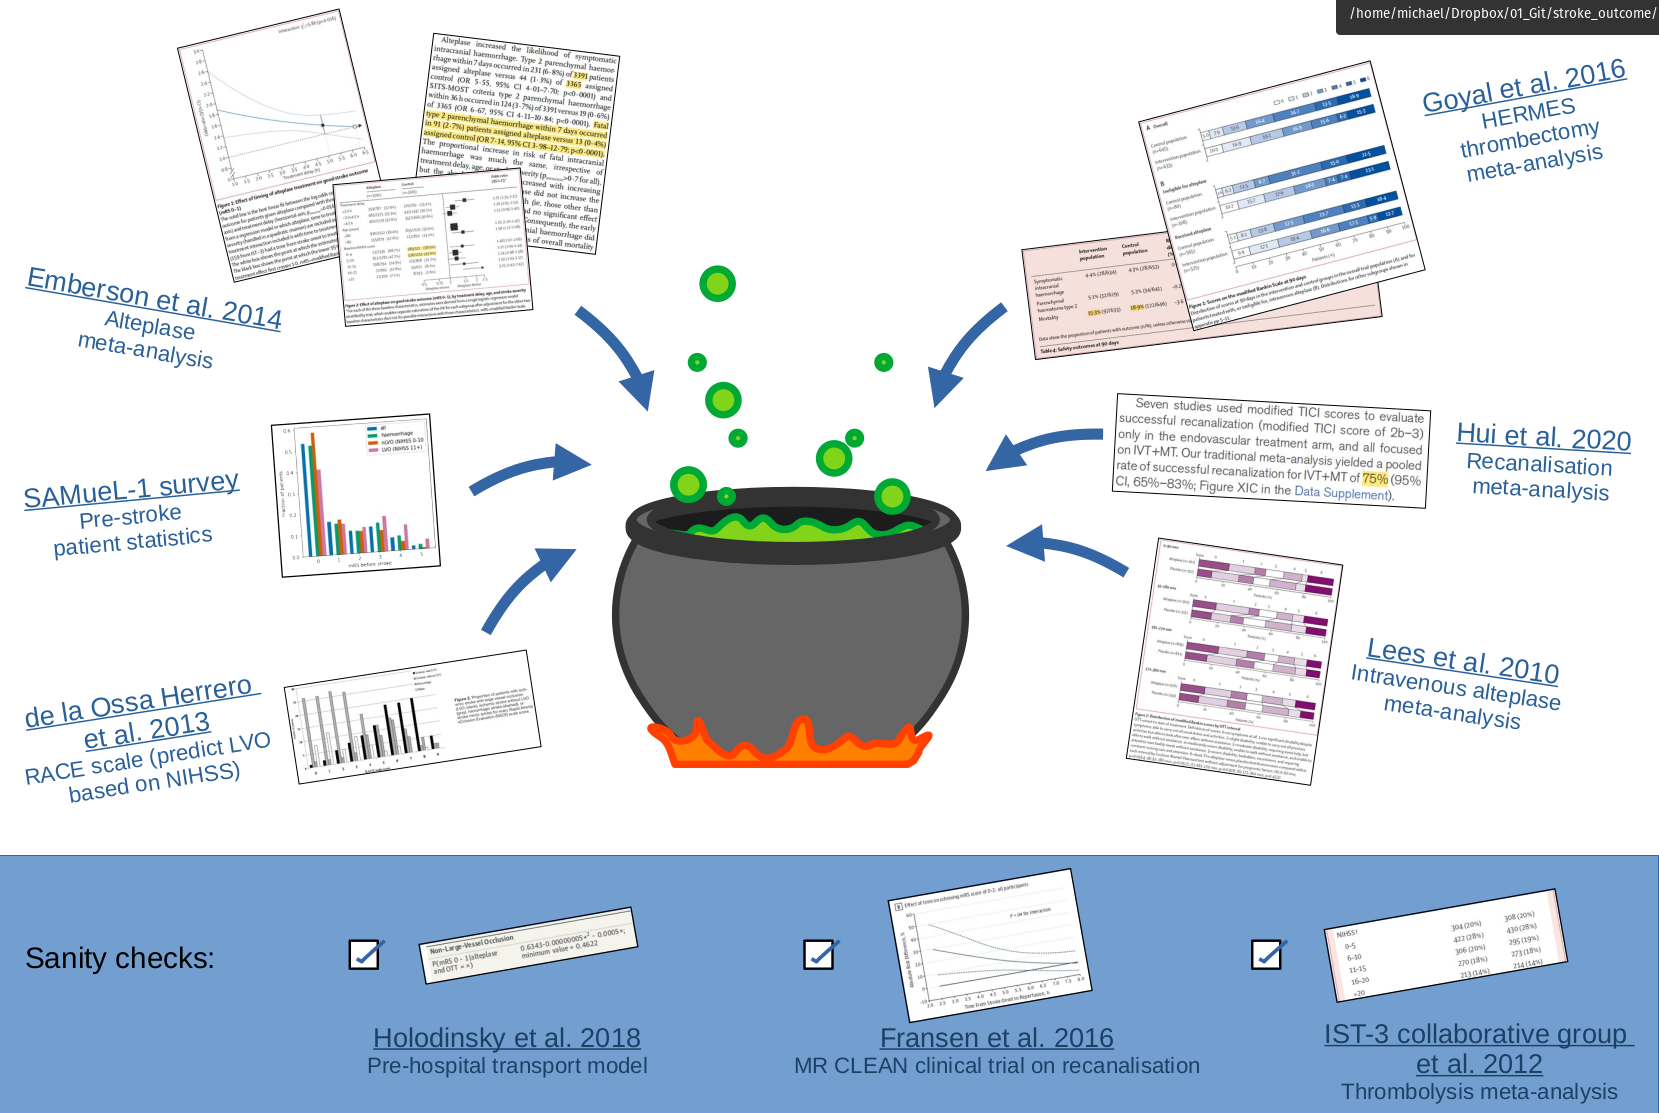
\includegraphics[width=1.0\linewidth]{images_modelling/data_cauldron.png}
    \caption{Depiction of hoe multiple data sources are combined to produce a mRS-level outcome model of nLVO and LVO stroke treated with thrombolysis and/or thrombectomy.}
    \label{fig:data_cauldron}
\end{figure}

The model results in mRS probability distributions for nLVO treated with IVT and LVO treated with either IVT or MT (figure \ref{fig:probs_with_time}).

\begin{figure}[h!]
    \centering
    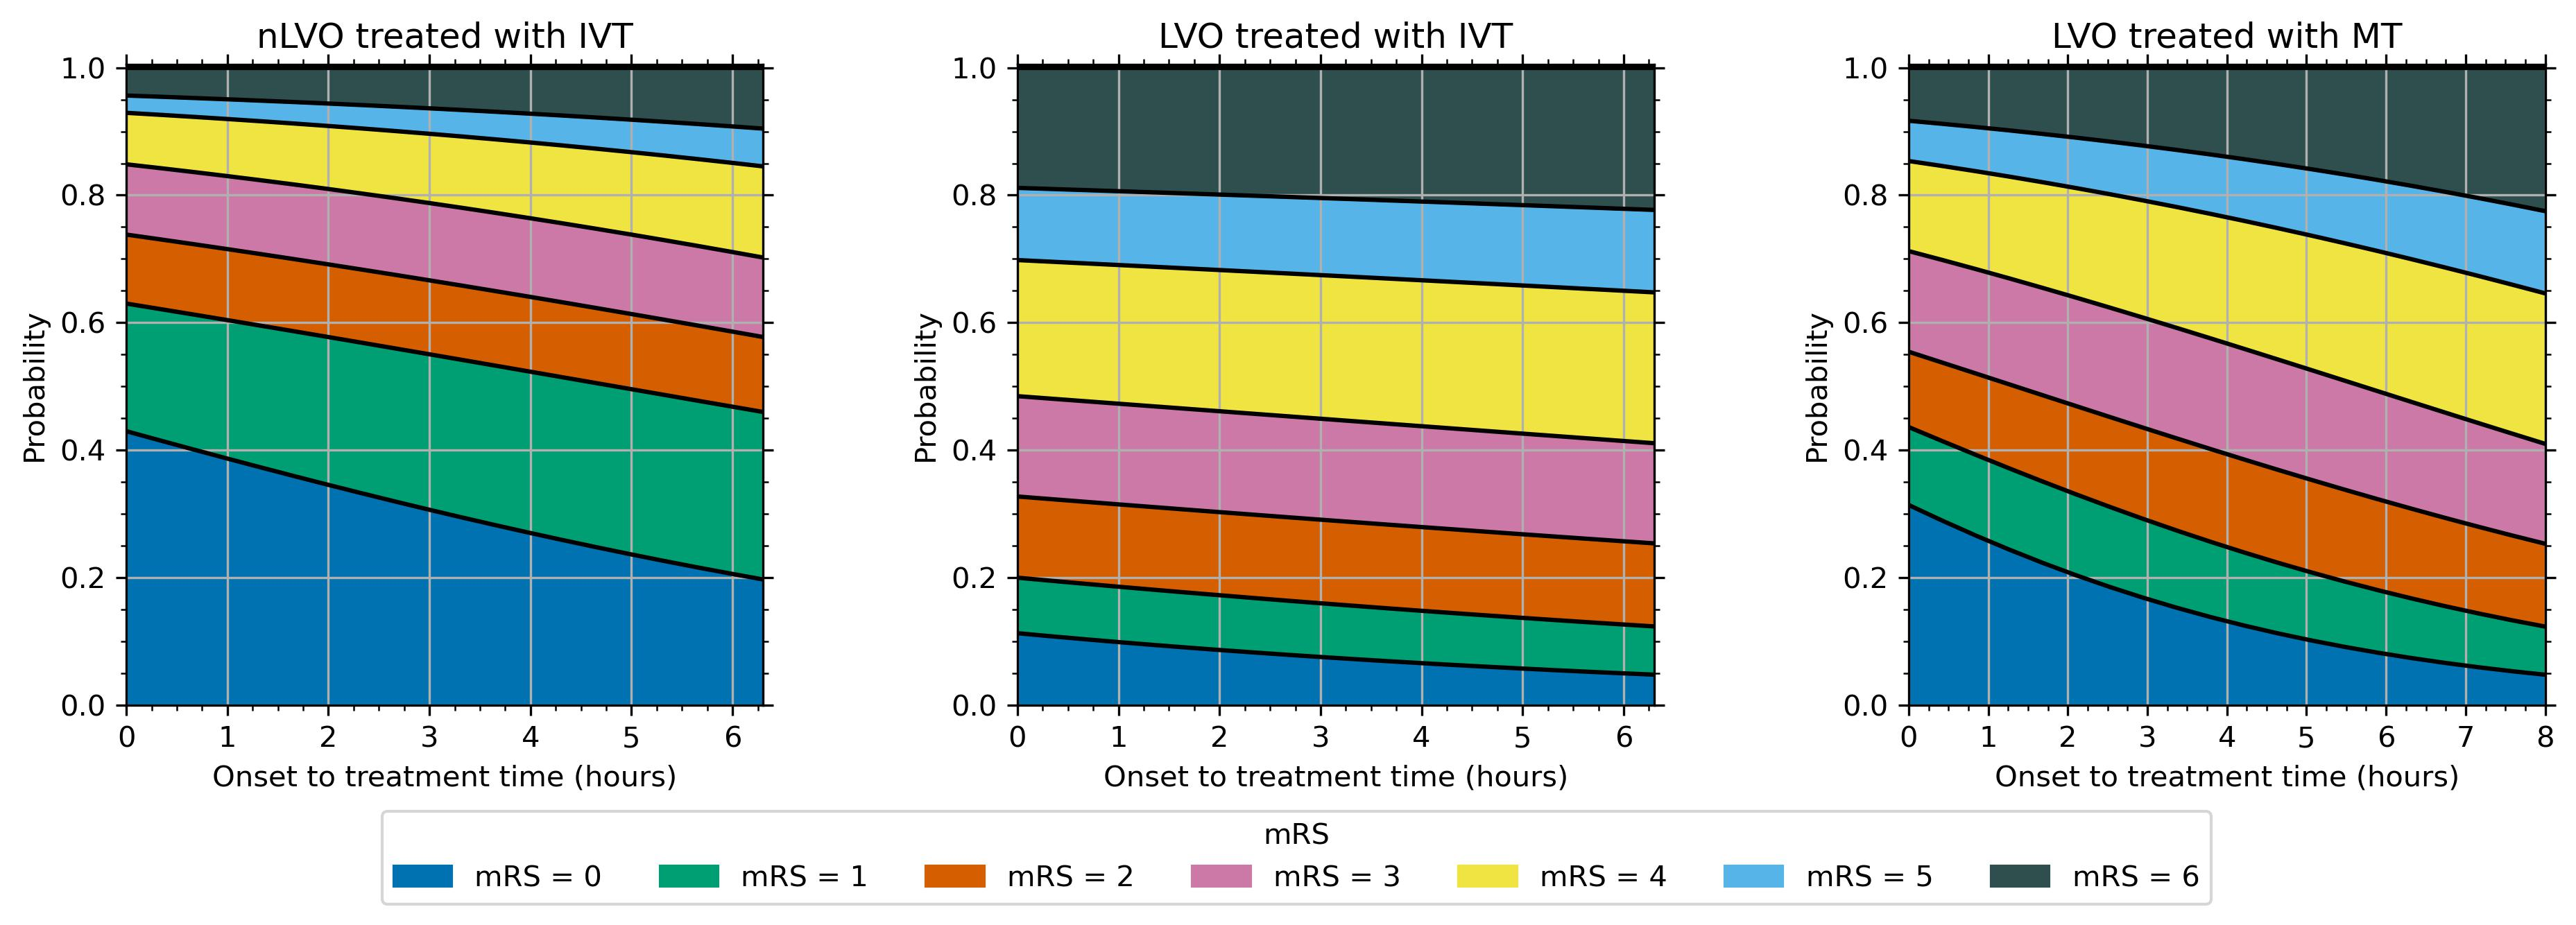
\includegraphics[width=1.0\linewidth]{images_modelling/probs_with_time.jpg}
    \caption{Final model predictions of mRS distributions for nLVO and LVO depending on time to treatment with IVT (for nLVO or LVO) or thrombectomy (for IVT and LVO).}
    \label{fig:probs_with_time}
\end{figure}

